\section{2D Merging}
\label{sec:2d_merging}

In the previous sections we have seen how to process individual images of 2D crystals. From a single micrograph we generate a list of spots containing their amplitudes and phases in Fourier space. This section describes how to merge the projection maps from each micrograph of an non-tilted specimen in order to produce one common projection map. This is similar to creating class averages in single particle electron microscopy, where projections of particles with the same orientation are averaged together.

In contrast to single particle classification in the context of 2D crystals we already know the projection direction from the electron microscope, all under the assumption that the crystals are perfectly flat. The central section theorem gives us the mathematical backbone to consider each image created by a transmission electron microscope as a projection of the crystal. Thus all images of non-tilted 2D crystals represent a projection of the crystal in z direction. In the previous section we have seen how filtering the Fourier transform of 2D crystal results equals averaging the proteins in real space. The task of 2D merging is to average the Fourier components of the images of untitled crystals together.

To be able to average the densities gained from each image one has to align the images first. They have to be in register with each other which is best done by aligning them to a common reference. As we see later in the practical part the reference is just one of the images chosen by the user. The alignment can also be understood as setting a common origin. 

We again make use of the Fourier theory for this task. For  single image processing we only considered at the amplitudes of the Fourier transform and the lattice it spans. This lattice always had a common origin and approximately the same dimensions, only the orientation varies across the images. This is due to that the magnitude of the Fourier Transform does not change even when the image is shifted. Therefore averaging the amplitudes is just averaging the diffraction spots with the same miller indices. The phases of the Fourier transform though determines the origin of the image in real space. Thus aligning all the images  results in shifting the phases of each image to match with the reference.

The last step of 2D merging is averaging. The simplest way would be to take the mean of the values for each unique reflection depicted by a Miller index. But the program \texttt{AVRGAMPHS} written by Richard Henderson weights each reflection based on its IQ value. Hence each single diffraction spot of every image contributes to the average according to its signal-to-noise ratio. For the user this has the advantage that even images of bad quality can be merged without making the resulting 2D map worse, additionally one can still benefit from the few spots that have a good IQ value. The final merged 2D map is then the inverse Fourier transform of the list of averaged amplitude and phases. 

\subsection{2D Merging in {\twodx}}

Having processed all the images of non-tilted specimen with {\twodx}\texttt{\_image} we are ready to merge them to an average projection map. As the name states we need {\twodx}\texttt{\_merge} for this task.

\begin{enumerate}
	\item If not already open, start up {\twodx}\texttt{\_merge} and select the project you want to work on.
	\item The parameter \textit{Modus of Merging}\index{Modus of Merging!2D}  has to be set to \textit{2D} in the "Processing Data" panel.
	\item We want to align the images to a common phase origin. Therefore we have to select one image as reference. Usually the image with the highest QVal and/or lowest phase residual error is used. The QVal can be read from the "QVal2" column in the project panel. To make it easier one can also sort the images by the this attribute by clicking on the title of the column as shown in \autoref{fig:2dx_merge_qval}.
	
	\begin{figure}[H]
		\centering
		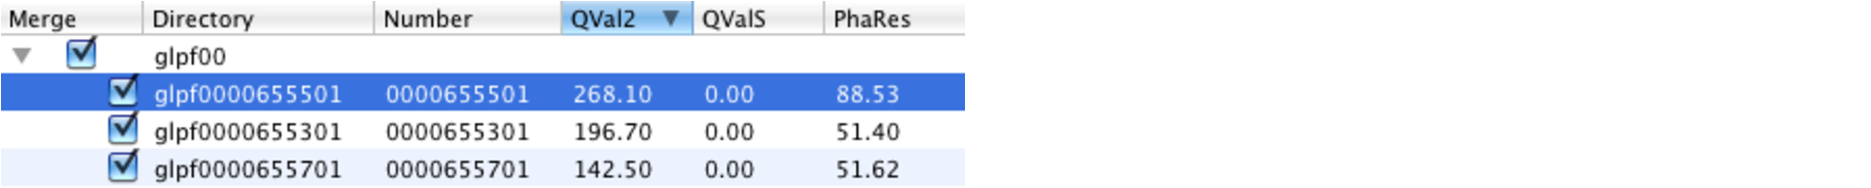
\includegraphics[width=0.85\textwidth]{2dx_merge_qval.pdf}
		\caption{Select the image with highest QVal as a reference.}
		\label{fig:2dx_merge_qval}
	\end{figure}

	\item  When choosing the reference make sure that the phase origin of the image was chosen accordingly the present space group (\autoref{sec:space_group}). If the image suffers from a wrong phase origin you should set the phase origin manually for the image as described in the phase origin section \autoref{sec:space_group}.
	\item The appropriate reference should be selected with the tick mark in the file panel. Make sure no other images are selected.
	\item Before creating the reference one should to chose the resolution the data on which the alignment process can rely on. This resolution is specified by the parameter \textit{Resolution of the merged dataset for the reference}. For the GLPF test data set we set this value initially to 15 \AA.
	\item Make sure the \textit{Symmetry} is set correctly in the processing data panel because the selected symmetry will be applied to the reference, i.e. correction of symmetry-restricted phase values and removal of symmetry-forbidden reflections.
	\item Now run the Standard Script \textit{Merge Once}. This script merges the data of the selected image into a reference file. Several output files are created as listed in the Images panel. The essential ones are the merge.aph, which is the list of merged amplitude and phases, and the MTZ file, which is then used as reference named \textit{MTZ: Merged full reciproc. space 2D data for reference}. Double clicking the MTZ file will show the content in your web browser. The file mainly consist of a reflection list as already seen in the APH file. Every reflection is depicted by there index (H,K,L), where the L is set to 0 in the 2D merging. Followed by amplitude and phase, which have been CTF corrected and symmetrized. The MTZ file also contains information about the crystal unit cell dimensions, the symmetry, the resolution range, etc.
\end{enumerate}

Now that we have created a  reference we can start aligning the non-tilted image data.

\begin{enumerate}
	\item Uncheck the image you have selected to be the reference and select all other images recorded from non-tilted specimen that you want to align.
	\item With the script \textit{Refine Once}\index{Refine Once} you can now align the selected images to the reference. All you need to do is to specify the range over which the phase origin search should be performed. Unless you have already manually selected the phase origin in all of the projection maps (\autoref{sec:space_group}) we advise you to initially cover the entire crystal unit cell i.e. a search range of 360{\textdegree} phase angle. The search range is defined by the parameters \textit{Stepsize of the phase origin search} and the \textit{Number of steps in the phase origin search} in the \textit{Merging} section. In a first phase origin search you should use a coarse step size of 6\textdegree~which with a number of 60 steps will go from -180\textdegree~to 174\textdegree. In later stages you should decrease the step size to a smaller value in order to perform a local refinement of the phase origin.
	\item Run the \textit{Refine Once} script. This will refine the phase origin for all selected images with the help of the MRC program \texttt{origtilt}. The last phase origin change for every image will be listed as \textit{phaori\_last\_change} in the Results panel as well as in the \textit{PhaOri Change} column of the Project panel.
	\item Now we visually inspect the phase origin change for each projection map by running the \textit{Generate Image Maps}\index{Generate Image Maps} script. Therewith the projection map are updated with the refined phase origin and is reflected in the Image Preview panel. You can scroll through the images in the Images panel or the Project panel. If you only want to see the selected images in the Project panel you can select the option \textit{Show Only Selected Directories} from \textit{View} menus illustrated in \autoref{fig:2dx_merge_menu_view_selected}. The same menu option can be used to switch back to view all images.
	
	\begin{figure}[H]
		\centering
		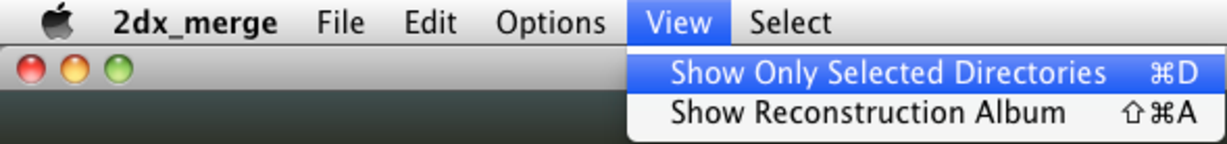
\includegraphics[width=0.85\textwidth]{2dx_merge_menu_view_selected.pdf}
		\caption{Shows only the selected images in the Project panel.}
		\label{fig:2dx_merge_menu_view_selected}
	\end{figure}
	
	\item Run \textit{Refine Once} again with the current step size until the phase origin of all refined images does not improve anymore. Depending on the step size it might happen that the optimal phase origin is in-between the two considered phase origins and will jump back and forth. This is also a sign that you have reached the optimum for this step size and should decrease it for the next merge and refinement runs.
	\item Besides the updated parameters in the results panel, the script also produces output files in the images panel. If you are curious how \texttt{origtilt} is called to refine every single image you should have a look at \textit{CSH: refinement script}. The output of \texttt{origtilt} might be more interesting and is in the text file listed as \textit{LOG: origtilt B output}. This file should be considered when evaluating the refinement process. It contains the list of reflections for all refined images. The most important value in this file though is the refined phase origin. It is followed by a table of resolution ranges with the associated phase residual for the reflections in that range. This allows the verification up to what resolution the refinement is trustworthy. One thing to keep in mind is that for the coarse refinement we limited the resolution of the reference. After the resolution table in \textit{LOG: origtilt B output} a cross-correlation map is plotted through a matrix where each entry represents the normalized cross-correltation value between the refined image and the reference. It should contain a clear peak which should end up in the center after the last rounds of refinement.
	\item After the first cycle of refinement we should update our reference with the refined data. Therefore include the image you initially used as a reference by adding it to the selection. Now run \textit{Merge Once} again to create a new reference. 
	\item If you set the \textit{Symmetry} in the Processing Data panel and the symmetry is above space group P2 you will get a table named "Phase Residual In Resolution Ranges". You should consider the phase residuals as measure to what resolution you can trust your data and adapt the \textit{Resolution of the merged dataset for the reference} accordingly. The resolution ranges of the table list the phase residual up to the \textit{Upper Resolution limit} plus 1\AA~further.
	\item With the new reference at hand we can preform a finer refinement of the phase origin. Hence the \textit{Stepsize of the phase origin search} should be decreased to e.g. 0.5\AA. In any case make sure that the step size together with the number of steps at least span the range of the previous step size (In our case 6\AA).
	\item Now run \textit{Refine Once} again for the refinement until the phase origin for each image does not change anymore i.e. \textit{PhaOri Change} will be zero. The cross-correlation maps in \textit{LOG: origtilt B output} should now show sharp and centered peaks.
	\item Until now we have always executed the merge and refine process separately. But when you are at the point where the images merged to a reference are the same set as the images being refined i.e. the selection does not change, you can also use the \textit{Merge \& Refine (Iterative)}\index{Merge \& Refine (Iterative)}  script. As the name states this runs several iterations of the merge and refine cycle by default 3 rounds. The iteration number can be changed by clicking as illustrated in \autoref{fig:2dx_merge_merge_refine_iterative}.
		
	\begin{figure}[H]
		\centering
		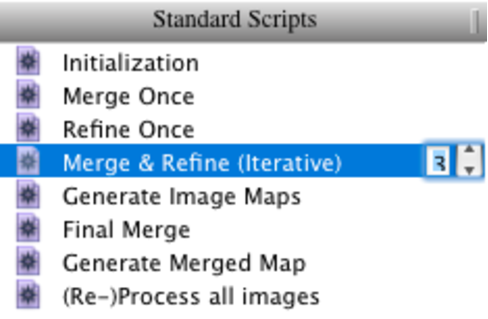
\includegraphics[width=0.5\textwidth]{2dx_merge_merge_refine_iterative.pdf}
		\caption{Changing the number of times the  \textit{Merge \& Refine} script is run by double clicking the counter.}
		\label{fig:2dx_merge_merge_refine_iterative}
	\end{figure}
	\item When using \textit{Merge \& Refine (Iterative)} script one should have a look at the parameters \textit{phaori\_last\_change} and \textit{MergePhaseResidual} in the Results panel like in \autoref{fig:2dx_merge_merge_results_params}. As we have mentioned before the phase origin change should decrease with each iteration and ideally end up being zero. The measure of how good the refined phase origin is quantified \textit{MergePhaseResidual}\index{Merge Phase Residual}. This value will also decrease in the process of refinement. If the value remains around 90\textdegree~then the alignment is not working.
		\begin{figure}[H]
		\centering
		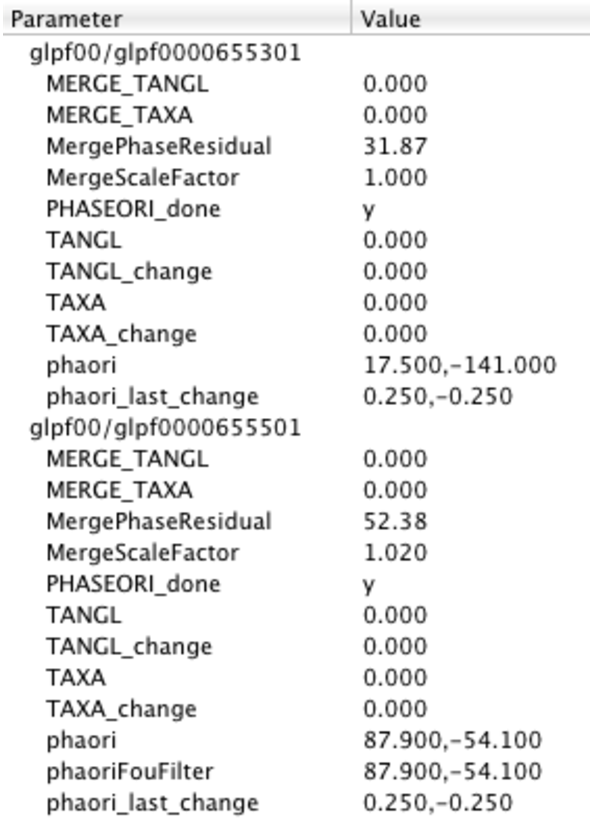
\includegraphics[width=0.5\textwidth]{2dx_merge_merge_results_params.pdf}
		\caption{The results of each refinement iteration is displayed as list of parameters for each image in the Results panel. The most important parameters to monitor are \textit{phaori\_last\_change} and \textit{MergePhaseResidual}.}
		\label{fig:2dx_merge_merge_results_params}
		\end{figure}
	\item For more in-depth knowledge about your merged data set there is the option \textit{List Reflections into logfile (ILIST)}\index{List Reflections into logfile (ILIST)}. If this is enabled a separate log-file is created called \textit{LOG: reflections after origtiltk}. This file is the complete list of reflections from every merged image. This means that for every H,K index the available values from the contributing images is listed. The values associated with each reflection besides the H,K index are the amplitude, phase, image number, IQ, film weight, background amplitude and CTF. Appending these values are dashed lines followed by the IQ value again. The number of dashed lines is inverse proportional to the IQ value i.e. a reflection with an IQ of 1 has the most dashed lines appended. This helps to identify the good reflections even in a large list. The reflections with IQ values of 1 to 4, even have the amplitude and phases repeated at the end. This should make it easier to detect reflections with data differing from the amplitude and phases of the same reflections stemming from other images. This deviation can be a sign for a wrong CTF correction in that image, therefore you should have a look if the defocus was detected correctly in this image. 
	\item If you did not add all the non-tilted images yet or have gained new images from the microscope you should use the existing reference to align the novel images in the same fashion by jumping back to step 1.
\end{enumerate}
Once all the data of the non-tilted images are aligned the last step is to merge them all together to one.
\begin{enumerate}
	\item As described above the final alignment should also be visually inspected by running the \textit{Generate Image Maps} script again and then scrolling through the images. An alternative to looking at the individual projection maps one by one in the  Image Preview panel is given by the \textit{Reconstruction Album}. The \textit{Reconstruction Album} shows for every image the projection map as thumbnail and when selected the image is shown large in the lower panel as illustrated in \autoref{fig:2dx_merge_reconstruction_album}. The album can be displayed in the View menu via \textit{Show Reconstruction Album}. Deselect the miss-aligned images.
	
	\begin{figure}[H]
		\centering
		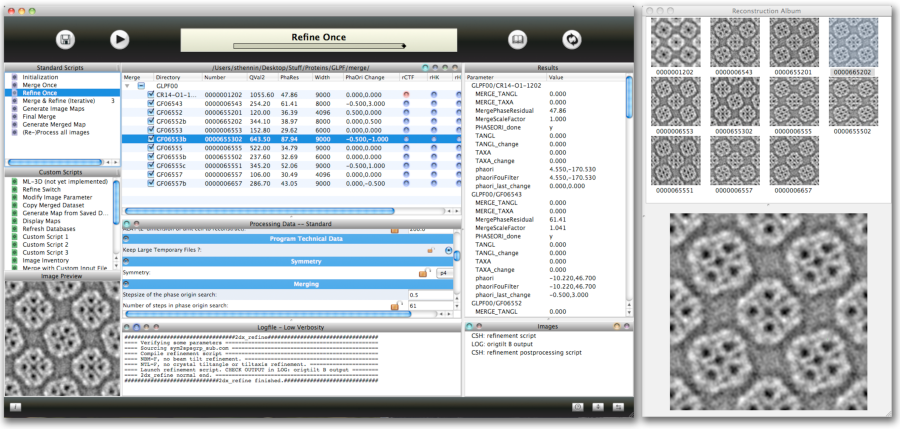
\includegraphics[width=1.0\textwidth]{2dx_merge_reconstruction_album.pdf}
		\caption{The Reconstruction Album gives an overview of the already processed images shows in form of projection map thumbnails and is a good alternative to the \texttt{2dx\_merge} interface on the left.}
		\label{fig:2dx_merge_reconstruction_album}
	\end{figure}
	
	\item Running the \textit{Final Merge}\index{Final Merge} script is similar to the previous merge steps, except that we will not use the result as a reference for further alignment, rather as resulting average 2D map. Hence it is of great importance to chose the \textit{Upper Resolution Limit (RESMAX)} carefully. One should only trust the data up to a resolution where the phase residual are low. If you are looking at the table of phase residuals a good estimate if phase residual reflects meaningful data can be given by the following relation
	\begin{equation}
		phase\,residual \leq 90^{\circ} - \dfrac{90^{\circ}}{\sqrt{n}}
	\end{equation}
	where $n$ is the number of spots in a given resolution range.
	\item The last step of 2D merging is to create a merged projection map through the \textit{Generate Merged Map}\index{Generate Merged Map} script. This creates two kind of 2D maps: one in form of an MRC image and the other in form of a contour plot. For our example data set where we set the symmetry to P4 and the files the images are named \textit{p4-symmetrized final 2D map} and \textit{PS: p4-symmetrized final 2D map plot}. The \textit{p4-symmetrized final 2D map} of the GLPF example data set should look similar to \autoref{fig:2dx_merge_merged_map}.
	
		\begin{figure}[H]
		\centering
		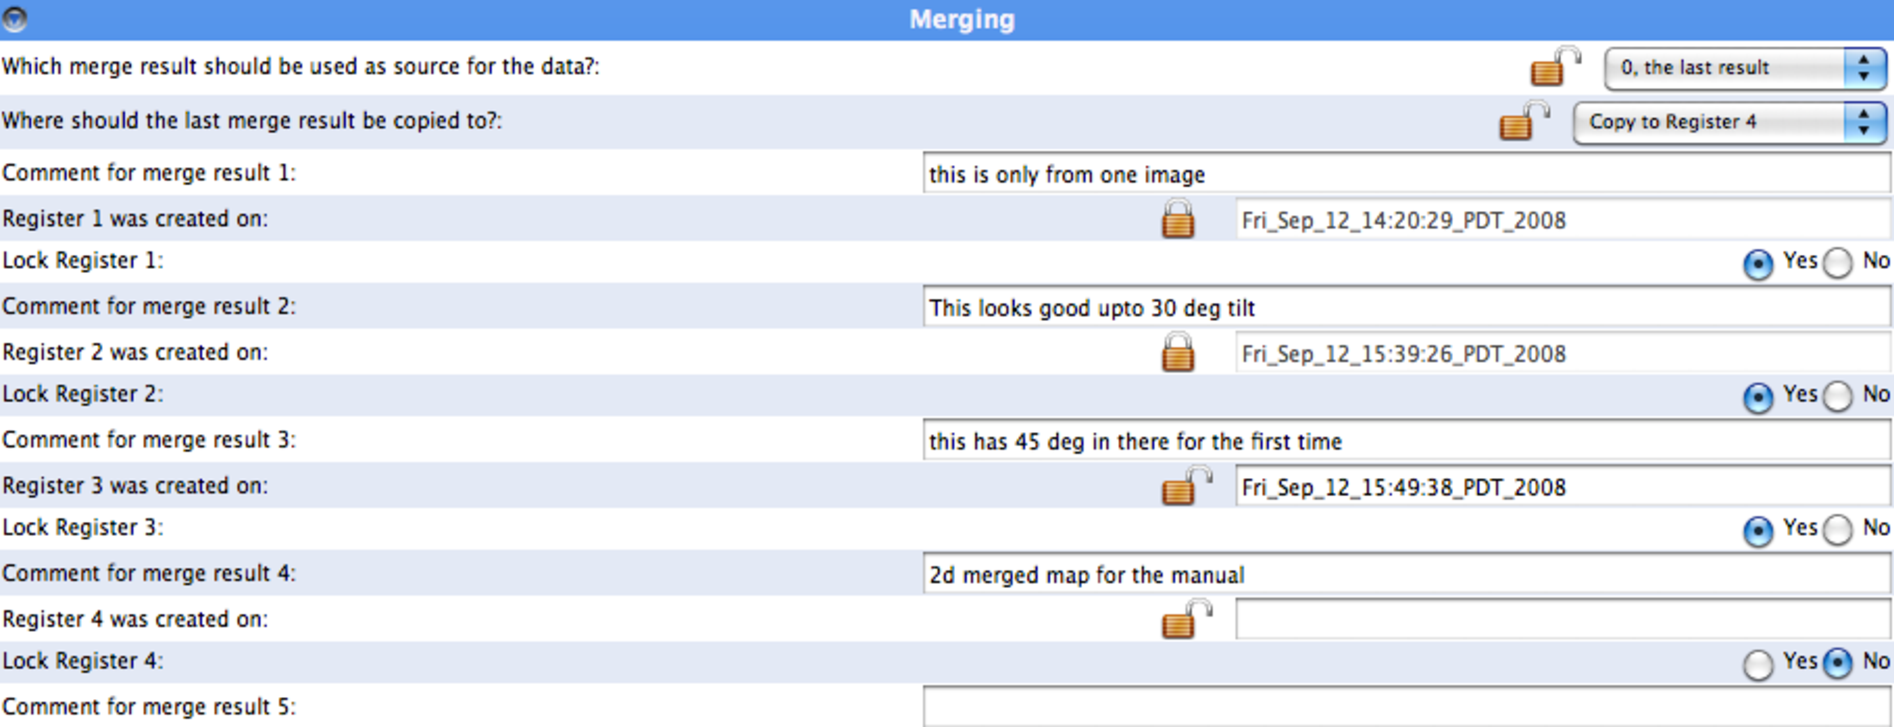
\includegraphics[width=0.8\textwidth]{2dx_merge_merged_map.pdf}
		\caption{The 2D merged map of the GLPF example data set.}
		\label{fig:2dx_merge_merged_map}
	\end{figure}
	
\end{enumerate} 



\subsection{Synthetic Unbending in {\twodx}}
\label{sec:syn_unbending}
\index{Synthetic Unbending in {\twodx}}

Once you obtained a first merged dataset you can go back and re-process all your single images. Your merged map represents so far the best model and can be used to create a "perfect" reference for unbending (see \autoref{sec:2dx_image}). This so called "synthetic reference" \index{synthetic reference} will be used in the \textit{Synthetic Unbend}\index{Synthetic Unbend} script in {\twodx}\texttt{\_image}.  \\ 
In order to re-process all images you have first to switch all selected images to \textit{Use Synthetic Reference}, by running the custom script \textit{Custom Script}\index{Custom Script} or \textit{Refresh Databases} \index{Refresh Databases} script in {\twodx}\texttt{\_merge}. Here you have to unlock the variable \textit{SYN\_Unbending to 1} as illustrated in \autoref{fig:unlockSynUnbend}.  

\begin{figure}[H]
		\centering
		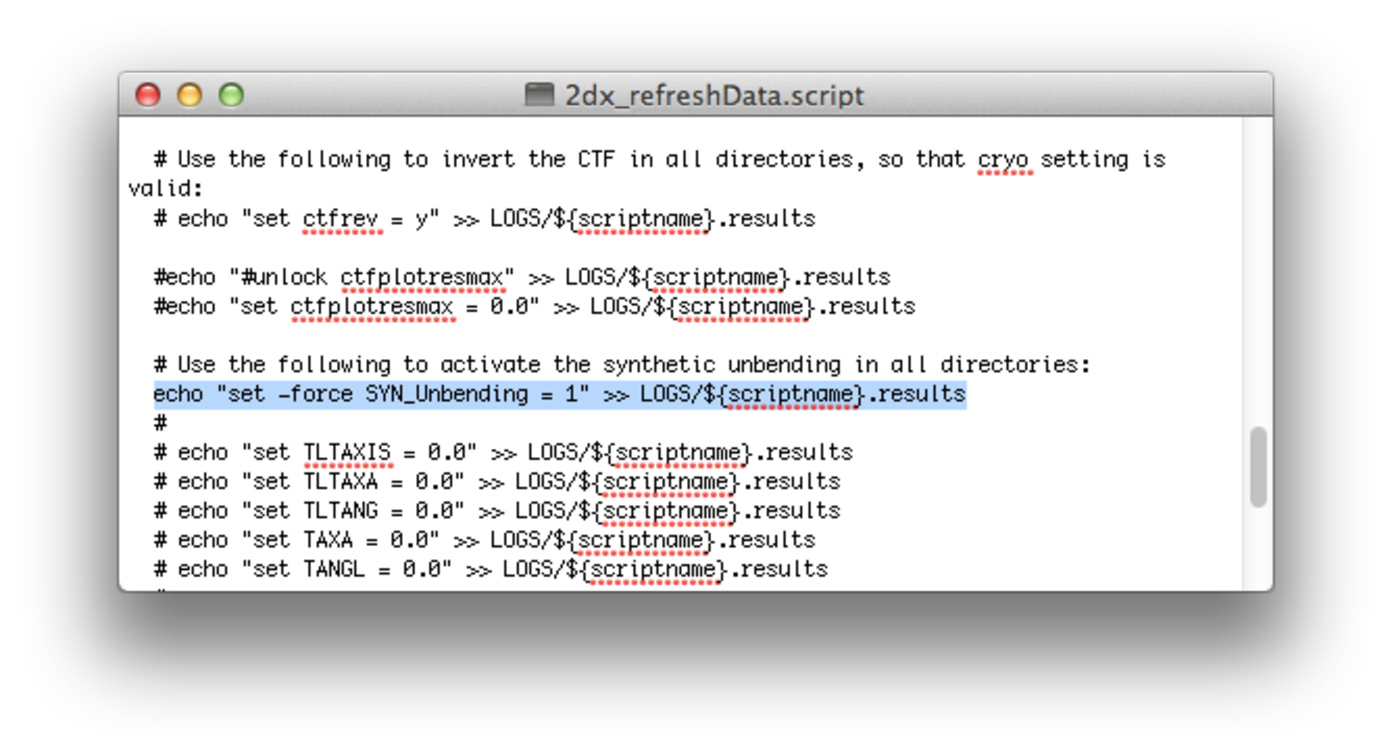
\includegraphics[width=0.8\textwidth]{unlockSynUnbend.pdf}
		\caption{How to select synthetic reference for all images.}
		\label{fig:unlockSynUnbend}
	\end{figure}
	
Now you can run the script \textit{Re-Process all Images}\index{Re-Process all Images} in {\twodx}\texttt{\_merge}, which will automatically rerun all required scripts including \textit{Synthetic Unbend}\index{Synthetic Unbend} as illustrated in the Logfile panel in \autoref{fig:reprocess}. Similar to Unbend I \& II, described in \autoref{sec:Unbend}, you can adjust the \textit{spot radius of the synthetical reference}.

\begin{figure}[H]
		\centering
		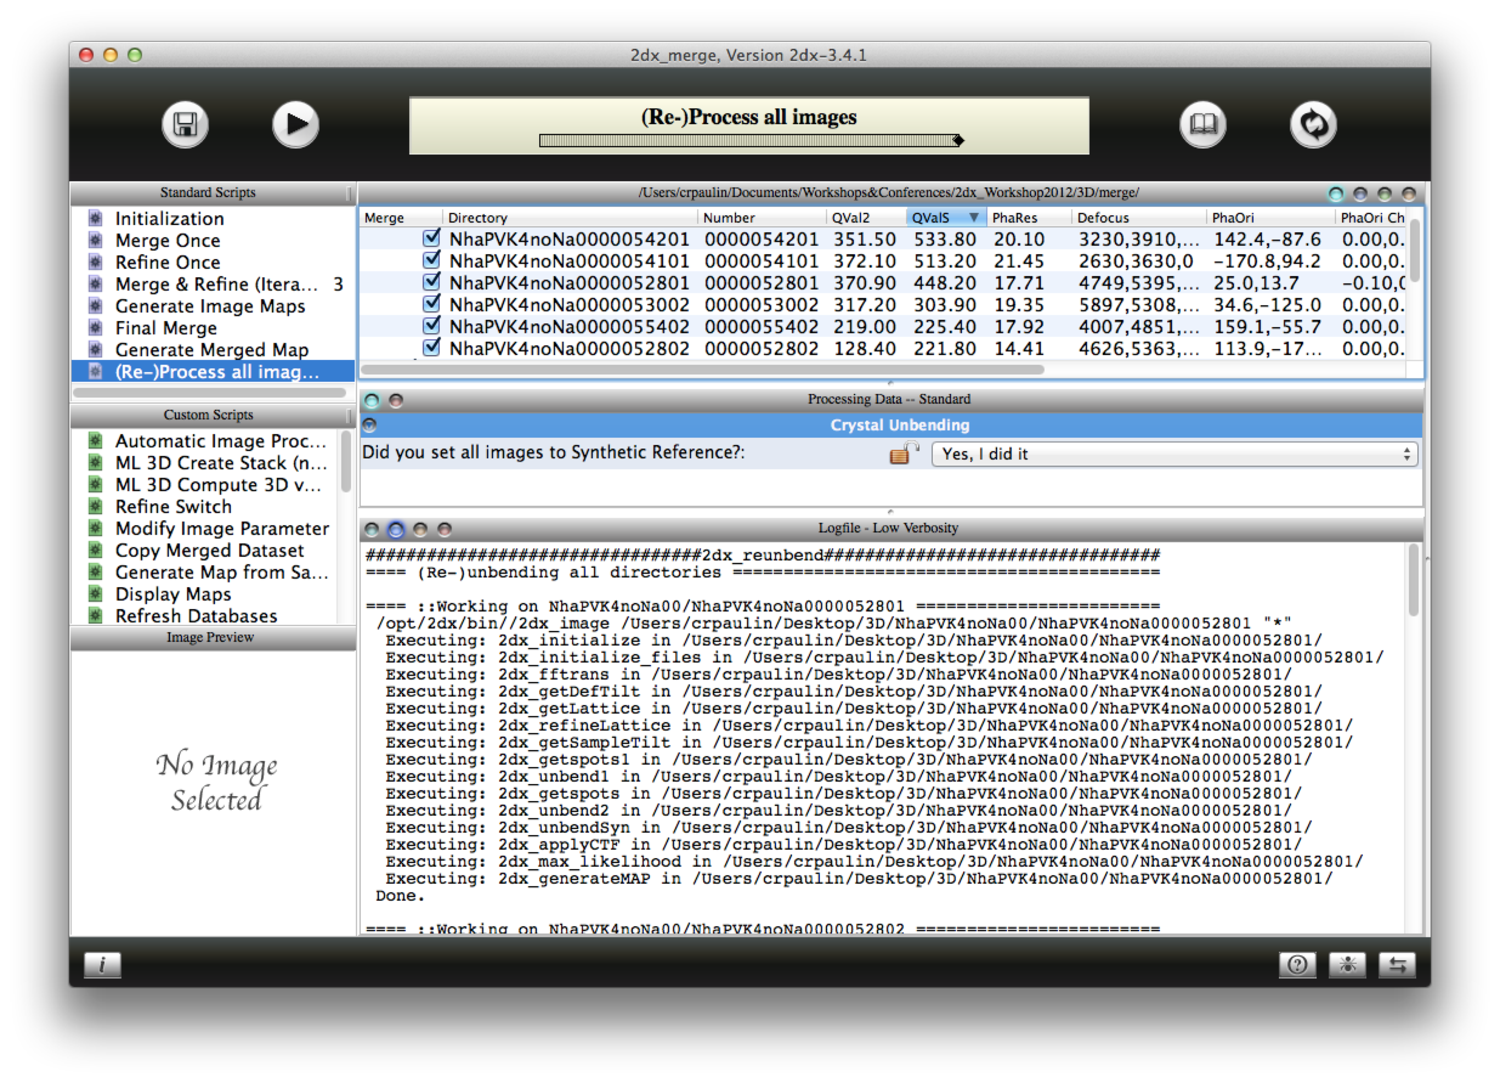
\includegraphics[width=\textwidth]{reprocess.pdf}
		\caption{Re-processing images with Synthetic Unbending in {\twodx}\texttt{\_merge}}.
		\label{fig:reprocess}
	\end{figure}
	

Reprocessing all images using a synthetical reference for unbending an image should lead to a significant improvement of the QVal values (here QValS) and of the phase residuals (see \autoref{fig:reprocess}). In some cases it also improves the resolution of your final merge map. Hence, \textit{Synthetic Unbend}\index{Synthetic Unbend} can be seen as a first refinement step for a merged dataset. 


